\data{16/03/2026} 
Stiamo dimostrando la correttezza parziale, per ogni funzione.
\paragraph{Correttezza parziale}Per ogni ingresso (valori dati ai parametri\footnote{ovvero gli argomenti.} durante la chiamata di funzione) che soddisfi la pre-condizione, \textbf{se la funzione termina}, allora la post-condizione è soddisfatta. 
\begin{figure}[tbph]
	\centering
	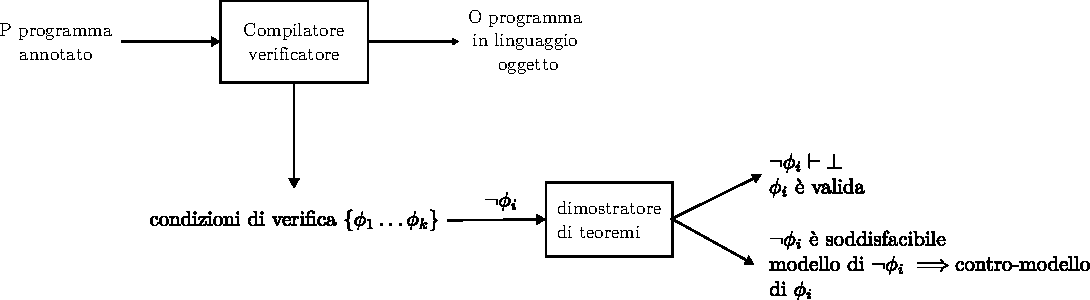
\includegraphics[width=\linewidth]{compilatore-verificatore-riepilogo-generale.pdf}
	\caption{un compilatore-verificatore che genera formule per il dimostratore di teoremi. Il dimostratore di teoremi risponde con una prova che $\phi_i$ è soddisfatta se da $\neg\phi_i$ si arriva ad una contraddizione, e risponde con un modello quando $\neg \phi_i$ è soddisfacibile da cui è possibile costruire un contro-modello di $\phi_i$. Questo serve per catturare gli stati del programma in cui $\phi_i$ è violata e dato che lo stato di un programma è l'assegnamento dei valori alle variabili del programma, è possibile ricavare informazioni utili per andare a correggere la logica del programma che causa la violazione di $\phi_i$ .}
\end{figure}

\begin{enumerate}
	\bitem{Annotazioni}includono le pre-condizioni, post-condizioni, \textbf{invarianti di ciclo} e asserzioni al runtime.
	\bitem{Cammini di base} i programmi contengono iterazioni e ricorsioni. Questa tecnica permette di decomporre il testo di un programma in cammini e fare l'analisi su ciascuno di essi. Un \textbf{cammino di base}\footnote{questa definizione va bene sia per l'iterazione che per la ricorsione.} inizia con una precondizione o un'invariante di ciclo e termina con una post-condizione o un'invariante di ciclo o un'asserzione di altro tipo. In mezzo ci sono istruzioni. 
	\begin{lstlisting}
§	\color{red}\textbf{Cammino di base}§
		§\color{blue}@F§  §\color{blue} $\rightarrow$ pre-condizione o invariante di ciclo§ 
		§$\begin{rcases}
			S_1;\\
			S_2;\\
			...\\
			S_n;
		\end{rcases}$§ istruzioni §\textit{assume}§ o assegnamenti alle variabili
		§\color{blue}@G§  §\color{blue}$\rightarrow$ post-condizione, invariante di ciclo o asserzione di altro tipo§
	\end{lstlisting}
\end{enumerate}
Le $S_1;...;S_n$ sono istruzioni \textit{assume} o assegnamenti alle variabili della funzione.
\subsubsection{Esempio di LinearSearch}

\begin{figure}[tbph]
	\centering
	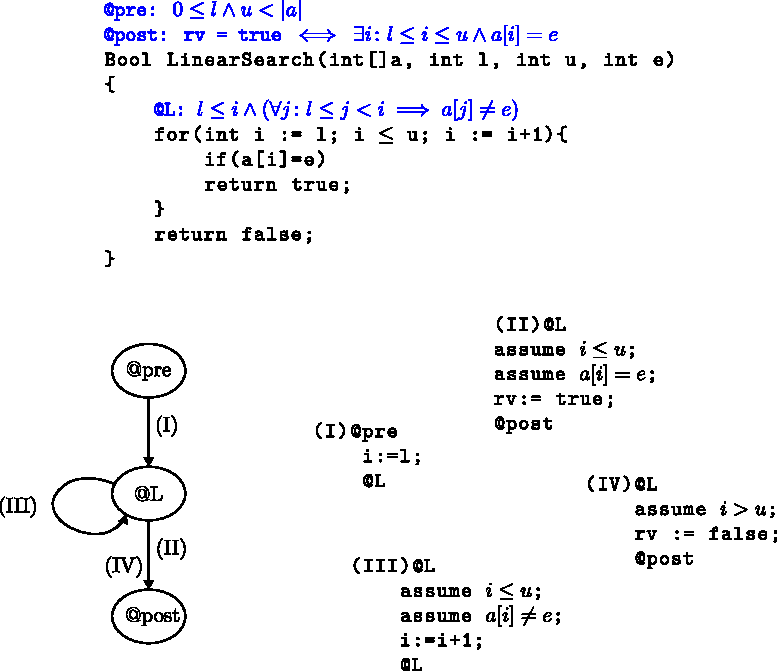
\includegraphics[width=.9\linewidth]{grafo-cammini-base}
	\caption{grafo dei cammini di base. Facendo riferimento all'invariante di ciclo \texttt{@L}, $\forall j\colon j<i$ perché dobbiamo ancora testare $i$. Bisogna verificare l''invariante interamente. Ad esempio nel caso di $l = i$ si ha che l'implicazione è vera perché la condizione sufficiente è falsa.}
	\label{fig:grafo-cammini-base}
\end{figure}
\begin{figure}[tbph]
	\centering
	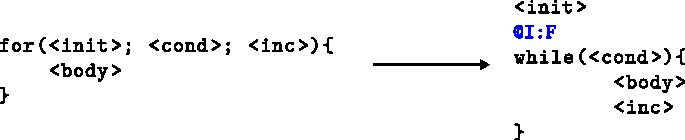
\includegraphics[width=0.7\linewidth]{trasformazione-for-in-while}
	\caption{trasformazione del for nel while.}
	\label{fig:trasformazione-for-in-while}
\end{figure}
Per costruire i cammini di base, prima si traduce il for nel while come in \cref{fig:trasformazione-for-in-while}, si fa una sorta di ``ricerca in profondità'', considerando le condizioni di ciclo e la condizione di guardia (\cref{fig:grafo-cammini-base}).
\hl{La decomposizione del programma in cammini di base è un attività automatizzabile.}

\paragraph{Trasformatore di predicato} Sia $L$ un linguaggio di formule. Un trasformatore di predicato è il prodotto cartesiano $$p\colon L\times \texttt{<stmts>}\longrightarrow L$$ dove \texttt{<stmts>} sono istruzioni. 
\paragraph{Weakest pre-condition} È un trasformatore di predicato, è una pre-condizione più debole che $$wp(F,S)$$ prende una formula e delle istruzioni e produce una formula. %58min
La $wp(F,S)$ è la pre-condizione più debole tale che $F$ è vera dopo aver eseguito $S$.
\paragraph{Stato del programma}È un assegnamento al PC\footnote{Program counter.} e a tutte le variabili e i parametri della funzione. Si estende in un'interpretazione. Sia $S\colon \text{stato del programma}$. Se siamo in uno stato $s\models wp(F,S)$ e $s\,S\,s'$ e $s'$ è stato del programma allora $s'\models F$.
\begin{figure}[thbp]
	\centering
	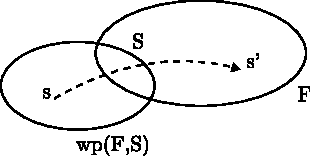
\includegraphics[width=0.45\linewidth]{wp}
	\caption{}
	\label{fig:wp}
\end{figure}

\begin{enumerate}
	\item $wp(F,\texttt{assume C})=C\implies F$\ \ \ \  $\inference{C\implies F\ \ \ C}{F}$ che è il modus ponens.
	\item $wp(F[x], x:=e)=F[x \leftarrow e]$
	\begin{itemize}
		\item $F[x]$: formula dove $x$ compare
		\item $F[x\leftarrow e]$: formula dove a $x$ si sostituisce $e$.
	\end{itemize}
	\item $wp(F, S_1;S_2)=wp(wp(F,S_2),S_1)$. Generalizzando $wp(F,S_1; ... ;S_n) = wp(wp(F,S_n),S_1;S_2;...;S_{n-1})$.
\end{enumerate}

Tornando ad un cammino di base generico
\begin{lstlisting}
	@F
	$S_1$
	$S_2$
	...
	$S_n$
	@G
\end{lstlisting}
qual'è la condizione di verifica per questo cammino? Si calcola la pre-condizione più debole $wp(G,S_1;...;S_n)$. La condizione di verifica sarà $$wp(G,S_1;...;S_n)\models F\implies wp(G,S_1;...;S_n)$$ che equivale a risalire il cammino da \texttt{@G} a \texttt{@F}.




